
%=================================================================
\documentclass{article}
%=================================================================

%------------------------------------------------------------------
% The following line should be uncommented if the LaTeX file is uploaded to arXiv.org
%\pdfoutput=1

%=================================================================
% Add packages and commands here. The following packages are loaded in our class file: fontenc, calc, indentfirst, fancyhdr, graphicx, lastpage, ifthen, lineno, float, amsmath, setspace, enumitem, mathpazo, booktabs, titlesec, etoolbox, amsthm, hyphenat, natbib, hyperref, footmisc, geometry, caption, url, mdframed, tabto, soul, multirow, microtype, tikz


\usepackage{listings}
\lstset{language=caml,basicstyle=\scriptsize,columns=fixed}
\usepackage{qtree}
\usepackage{tkz-graph}  
\usepackage{subcaption}
\usepackage{acronym}
\usepackage{todonotes}
\usepackage{algorithmicx,algpseudocode,algorithm}
\usepackage{amsmath,amssymb}
\usetikzlibrary{shapes.geometric,positioning,fit,backgrounds}
%=================================================================
%% Please use the following mathematics environments: Theorem, Lemma, Corollary, Proposition, Characterization, Property, Problem, Example, ExamplesandDefinitions, Hypothesis, Remark, Definition
%% For proofs, please use the proof environment (the amsthm package is loaded by the MDPI class).

%=================================================================
% Full title of the paper (Capitalized)
%\Title{A model for interactive media authoring}

% Author Orchid ID: enter ID or remove command
\newcommand{\orcidauthorA}{0000-0003-1253-298X} % Add \orcidA{} behind the author's name
%\newcommand{\orcidauthorB}{0000-0000-000-000X} % Add \orcidB{} behind the author's name

% Authors, for the paper (add full first names)
%\Author{Jean-Michaël Celerier $^{1,\dagger,\ddagger}$\orcidA{}, Myriam Desainte-Catherine $^{1,\ddagger}$ and Bernard Serpette $^{2,}$*}

% Authors, for metadata in PDF
%\AuthorNames{Jean-Michaël Celerier, Myriam Desainte-Catherine and Bernard Serpette}

% Affiliations / Addresses (Add [1] after \address if there is only one affiliation.)
%\address{%
%    $^{1}$ \quad Affiliation 1; e-mail@e-mail.com\\
%    $^{2}$ \quad Affiliation 2; e-mail@e-mail.com}
%
% Contact information of the corresponding author
%\corres{Correspondence: e-mail@e-mail.com; Tel.: +x-xxx-xxx-xxxx}

% Current address and/or shared authorship
%\firstnote{Current address: Affiliation 3} 
%\secondnote{These authors contributed equally to this work.}
% The commands \thirdnote{} till \eighthnote{} are available for further notes

% Simple summary
%\simplesumm{}

% Abstract (Do not insert blank lines, i.e. \\) 
%\abstract{A single paragraph of about 200 words maximum. For research articles, abstracts should give a pertinent overview of the work. We strongly encourage authors to use the following style of structured abstracts, but without headings: 1) Background: Place the question addressed in a broad context and highlight the purpose of the study; 2) Methods: Describe briefly the main methods or treatments applied; 3) Results: Summarize the article's main findings; and 4) Conclusion: Indicate the main conclusions or interpretations. The abstract should be an objective representation of the article, it must not contain results which are not presented and substantiated in the main text and should not exaggerate the main conclusions.}

% Keywords
%\keyword{interactive scores; intermedia; dataflow; patcher; i-score}

% The fields PACS, MSC, and JEL may be left empty or commented out if not applicable
%\PACS{J0101}
%\MSC{}
%\JEL{}


%\featuredapplication{Authors are encouraged to provide a concise description of the specific application or a potential application of the work. This section is not mandatory.}

\acrodef{DAG}{Directed Acyclic Graph}

\newcommand\mg[1]{\ensuremath{ {\boldsymbol<} #1 {\boldsymbol>} }}
\DeclareMathOperator{\tc}{TC}
\DeclareMathOperator{\ic}{IC}
\DeclareMathOperator{\itv}{I}
\DeclareMathOperator{\proc}{P}

\newcommand{\includecode}[2][c]{\lstinputlisting[caption=#2, escapechar=]{#2}<!---->}
\title{A model for interactive media authoring}
\begin{document}

\section{Introduction}
Many music software fit in one of three categories: sequencers, patchers, and textual programming environments. Sequencers are used to describe temporal behaviours: an audio clip plays after another, while an automation curve changes an audio filter. Patchers are more commonly used to describe invariants: for instance specific audio filters, or compositional patterns. 

We propose in this paper a method that combines the sequencer and the patcher paradigm in a live system.  

The general approach is as follows: we first introduce a minimal model of the data we are operating on: namely, remote software or hardware such as OSC peripherals and sound cards. Then, two structures are presented: the first is a temporal structure, which allows to position events and processes relatively to each other, hierarchically, and in a timely fashion. The second is a graph structure akin to dataflows. This graph uses special connection types to take into account the fact that nodes of the graph might not always be active at the same time. Both structures are then combined: the state of the temporal processes is bound to the dataflow nodes. This combination is then expanded with specific implicit cases that are relevant in computer music workflows. These cases are described using structures wrapping the temporal and dataflow graphs. 

We compare the various models in the context of music creation: what entails using only the temporal structure, only the graph structure, and the combination of both. 

The latter model is shown to have enough expressive power to allow for recreation of common audio software logic within it: for instance traditional or looping audio sequencers. Additionnally, its use is presented in sample compositions: the first one is an example of audio editing, the second an interactive musical installation.

% Ce qui manque: déclaration de variables locales pour nommage ? Actuellement on utilise des variables globales si on veut un nom.

% => décrire requirements pour qu'un autre système de contraintes temporelles puisse fonctionner 
% => au minimum : enable / disable

%Pbq si on fait ça en fonctionnel: construction obligatoire en "top-down" ? on commence par les processus, puis les contraintes, etc. 
% sinon on doit parcourir tout pour remplacer ce qu'on veut

% TODO audio : plutôt que stocker du std::vector<std::vector<float>> pourquoi pas un gsl::span<gsl::span<float>>

% Sample accuracy pour audio ? on pourrait faire un tick par échantillon au prix de la performance. Mais pb avec PureData, etc. qui veulent 64 samples: il faudrait un mécanisme de buffering...
% Changements de vitesse: introduire des noeuds de "rescaling"  dès qu'on a deux objets qui sont en relation et peuvent avoir une vitesse différente. eg deux processus 
\subsection{State of the art}

There is a long-standing interest in the handling of time in programming languages, which is intrinsically linked to how the language handles dynamicity.

PEARL90\cite{halang2001safe}\footnote{Not to be mistaken with the Perl language commonly used for text processing} provides temporal primitives allowing for instance to perform loops at a given rate for a given amount of time.
More recently, Céu has been introduced as a synchronous language with temporal operators, and applications to multimedia\cite{Santos:2016:CLI:2976796.2976856}.

OpenMusic is a visual environment which allows to write music by functional composition.
It has been recently extended with timed sequences allowing to specify evolutions of parameters in time\cite{garcia:hal-01484077}.

Likewise, the Bach library for Max~\cite{agostini2015max} allows to define temporal variations of parameters during the playing of a note by with the mechanism of slots.
The processes controlled by such parameters are then available to use in the Max patch.

The Max for Live extension to Ableton Live allows to embed Max patches in the Ableton Live sequencer. 
Through the API provided, one can control the execution of various elements of the sequencer in Max; automations in Live can also be used to send data to Max patches at a given time.

A method for dynamic patching of Max abstractions based on CommonLisp has been proposed by Thomas Hummel\cite{hummel1994common} to reduce resource usage by enabling and disabling sub-patches at different points in the execution of a program.
This has the advantage of saving computing power for the active elements of the score.

Dataflows and especially synchronous dataflows have seen tremendous usage in the music and signal processing community. 
A list of patterns commonly used when developing dataflow-based music software is presented in~\cite{arumi2006dataflow}.
Formal semantics are given in~\cite{benveniste_data-flow_1993}.
Specific implementation aspects of dataflow systems are discussed in the Handbook of Signal Processing Systems\cite{bhattacharyya_handbook_2013}. 

Dynamicity in dataflows is generally separated in two independent aspects: dynamicity of the data, and of the topology.
The first relates to the variability on the streams of tokens, while the second is about changes to the structure of the graph. 
Boolean parametric dataflows\cite{bempelis2015boolean} have been proposed to solve dynamicity of topology, by introducing conditionals at the edges.

base: max, pd, séquenceurs: cubase/protools , live/bitwig...

openmusic

antescofo

inscore


\subsection{Context of this research}
This paper follows existing research on interactive scores, as part of the i-score project.
Previous research focused on operational semantics for interactive scores, based on time automatas\cite{arias2016authoring} or Petri nets\cite{allombert2007system}, mainly for software verification purposes. 
In contrast, we give here domain-centered functional semantics which models the current C++ implementation of the software.

We first define the temporal model, then extend it with a distinct data model which reads and produces the various inputs \& outputs of the system. 
Then, we introduce implicit operations and defaults in the context of a GUI software to create, modify, and playback such scores. These operations allow to simplify the usage of the paradigm for composers.
Real-world examples are provided and discussed.

\cite{celerier2017icmc}

\section{Proposed sequencer behaviour}
We give here an overview of the whole system ; the choices and ideas proposed will be explained in detail in the following sections.

The overall goal is to associate traditional dataflow graphs with temporal semantics.
In terms of model, three structures are present: 
\begin{itemize}
    \item A global environment in the form of a tree of parameters. 
          It represents external software and hardware such as sound cards, MIDI controllers or OSC-compliant software
    \item The dataflow graph which will generate and process musical data
    \item The temporal graph which will specify when and how the dataflow graph runs.
\end{itemize}

For the dataflow graph, the traditional musical programming patterns of \todo{cite control-signal separation} and \todo{cite audio processing in buffers} are used.

The temporal graph allows three things :
\begin{itemize}
\item Embedding interaction choices in the time-line.
\item Arbitrary hierarchy.
\item Merging of loop-based and timeline-based control: we show in section\ref{sec.existingparadigms} that this is enough to allow both time-based and loop-based behaviors to co-exist in a single structure and user interface, unlike existing approaches which splits those in two mostly distinct domains ; this enables a large array of possible intermediary behaviors.
\end{itemize} 

Then, at each tick, the temporal graph runs as described in section~\ref{sec.temporal}.
This produces tokens in the dataflow graph nodes. 
Once tokens have been produced for every temporal structure, the data graph runs.
Graph nodes which did not receive any token for a given tick will not be executed.

To accommodate for the temporal semantics, dataflow semantics are extended with : 
\begin{itemize}
    \item The ability to specify input and output addresses to ports. 
          This allows nodes to read and write directly from the global environment, in a specified way and can be used to leverage type information associated with the parameters.
    \item Special connection types between edges to leverage the fact that not all nodes may be running at the same time.
\end{itemize}
 
When the graph runs, nodes read and write from their input and output ports ; relevant values are then copied in other ports or in the environment by the supervising algorithm.

The environment is separated in two parts: a local part which can serve to reuse the result of given computations in further node executions, and a global part which maps to messages sent to external devices.

For the sake of simplicity, the user interface merges the temporal and the data graphs in a single view. 
Section~\ref{sec.together} presents in detail some automatic set-up and enforced assumptions done by the software.

\begin{figure}
    \centering
    \begin{subfigure}[t!]{0.45\textwidth}
        \centering
        \small\def\qtreeunaryht{2ex}
        \Tree [.interval~I_0
        [.scenario 
        [.interval~I_1 mapping ] 
        [.interval~I_2 [.loop [.interval automation ] ] ] 
        interval~I_3 
        [.interval~I_4 sound ] 
        [.interval~I_5 effect ]
        ] 
        !\qsetw{1mm}  automation sound  ]
        \caption{Hierarchical tree}
    \end{subfigure}

    \begin{subfigure}[t!]{0.45\textwidth}
        
        \centering
        \tikzstyle{VertexStyle}=[
        shape=ellipse,
        minimum width=6ex,
        draw
        ]
        
        \tikzstyle{EdgeStyle}=[
        ->,
        >=stealth'
        ]
        \tikzstyle{EditTimeSync}=[
        rounded corners=.15cm, 
        fill=gray!30, 
        draw=gray, 
        fill opacity=0.3
        ]
        \tikzstyle{WaitTimeSync}=[
        rounded corners=.15cm, 
        fill=orange!30, 
        draw=orange, 
        fill opacity=0.3
        ]
        
        \begin{tikzpicture} 
        \pgfdeclarelayer{box}
        \pgfdeclarelayer{text}
        \pgfsetlayers{box,text}
        \begin{pgfonlayer}{text}
        \SetGraphUnit{1.5} 
        \Vertex[L=$\ic_1$]{C1} \EA[L=$\itv_1$](C1){I1} \EA[L=$\ic_2$](I1){C2} \EA[L=$\itv_4$](C2){I4}
        \SO[L=$\ic_3$](C1){C3} \EA[L=$\itv_2$](C3){I2} \SOEA[L=$\ic_5$](I4){C5}
        \SOEA[L=$\itv_3$](C3){I3} \EA[L=$\ic_4$](I3){C4} \EA[L=$\itv_5$](C4){I5}
        
        \Edges(C1, I1, C2, I4, C5)
        \Edges(C3, I2, C2)
        \Edges(C4, I5, C5)
        \Edges(C3, I3, C4)
        \end{pgfonlayer}
        
        \begin{pgfonlayer}{box}
        \node[fit=(C1) (C3), EditTimeSync, label=above:$\tc_1$] {};
        \node[fit=(C2), EditTimeSync, label=above:$\tc_2$] {};
        \node[fit=(C4), EditTimeSync, label=above:$\tc_3$] {};
        \node[fit=(C5), EditTimeSync, label=above:$\tc_4$] {};
        \end{pgfonlayer}
        \end{tikzpicture}
        
        \caption{Temporal DAG corresponding to the scenario}
    \end{subfigure}
\end{figure}
% TODO représenter trace d'exécution

\section{Orchestrated data}\label{sec.device}
We first define the data we operate on.
External devices are modeled as a tree of optional parameters.

Value parameters can have values of common data types such as integer, float, etc.
Audio parameters are arrays that contain either the current input audio buffers of the sound card or the buffers that will be written to the sound card's output.

The tree of nodes is akin to the methods and containers described in the OSC specification.

\begin{align*}
\mathbf{Value} & = \mathrm{Float} \mid \mathrm{Int} \mid \mathrm{Bool} \mid \mathrm{String} \mid \dots \\
\mathbf{ValueParameter} & = \mathrm{Value} \times \mathrm{Protocol} \\
\mathbf{AudioParameter} & = \mathrm{Float[][]} \times \mathrm{Protocol} \\
\mathbf{Parameter} & = \mathrm{ValueParameter} \mid \mathrm{AudioParameter} \\
\mathbf{Node} & = \mathrm{String} \times \mathrm{Maybe}~\mathrm{Parameter} \times \mathrm{Node[]} 
\end{align*}

Parameters and nodes bear additional metadata which is not relevant to describe here: textual description, tags, etc.

The parameters's associated values match the state of an external device: synthesizer, etc.
Multiple protocols are implemented to allow this: for instance OSC, MIDI, etc.

We define two core operations on parameters: 
\begin{align*}
\mathbf{pull} & : \mathrm{Parameter} \rightarrow \mathrm{Parameter} \\
              & (v, p) \mapsto (v', p)~\text{where v' is the last known value in the remote device}\\
\mathbf{push} &: \mathrm{Parameter} \times \mathrm{Value} \rightarrow \mathrm{Parameter} \\
              & (v, p), v' \mapsto (v', p)~\text{and v' is sent to the remote device} 
\end{align*}

\section{Temporal model}\label{sec.temporal}
The temporal model is twofold: it is a hierarchical tree of processes, whose durations and execution times are directed by intervals organized in a \ac{DAG}. 
The beginning and end of the intervals is subjected to various conditions that will be presented ; these conditions allow for various 
interactive behaviors. Processes represent various kinds of relevant artistic process: automations, notes sequences, sound files ; they are unrelated to the process concept in operating systems. 
In particular, specific dispositions of intervals and conditions are implemented as processes themselves, scenario and loop, which allows for hierarchy.

We note: $\tc$ for temporal conditions, $\ic$ for instantaneous conditions, $\itv$ for intervals, $\proc$ for processes. 
First, these elements are defined, then the semantics imposed on them by the scenario and the loop are presented.
These semantics allow both serial and parallel execution of musical processes.

\subsection{Data types}   
    
\subsubsection{Conditions and expressions}
We first define the conditional operations we want to be able to express.
We restrain ourselves to simple propositional logic operands: \textbf{and}, \textbf{or}, \textbf{not}.

Expressions operate on addresses and values of the device tree presented in \ref{sec.device}.

Formally, expressions are defined as a tree:
Let \textbf{Comparator} be an identifier for standard value comparison operations: $<, \leq, >, \geq, =, \neq$ and \textbf{Operator} standard logical operators \textbf{and} \&  \textbf{or}.

\begin{lstlisting}
type subexpr = Var of string | Value of value;;
type expression =
| Greater   of subexpr*subexpr
| GreaterEq of subexpr*subexpr
| Lower     of subexpr*subexpr
| LowerEq   of subexpr*subexpr
| Equal     of subexpr*subexpr
| Different of subexpr*subexpr
| Negation  of expression
| And       of expression*expression
| Or        of expression*expression
| Impulse   of impulseId*string
;;
\end{lstlisting}
Two operations are defined on expressions and the data types that compose them: 

%\begin{itemize}
%    \item $\mathbf{update}: \mathrm{Expression} \rightarrow \mathrm{Expression}$. Used to reset any internal state and query up-to-date values for the expressions. For instance, $\mathbf{update}$ on an $\mathbf{Atom}$ fetches if possible new values for the parameters, why may include network requests.
%    
%    Precisely:
%    \[
%    \begin{cases}
%    \mathrm{update} : & \mathrm{Composition} \rightarrow \mathrm{Composition} \\ 
%    & (e_1, e_2, o) \mapsto (\mathrm{update}~e_1, \mathrm{update}~e_2, o) \\
%    \mathrm{update} : & \mathrm{Negation} \rightarrow \mathrm{Negation} \\
%    &  e_1 \mapsto \mathrm{update}~ e_1 \\
%    \mathrm{update} :&  \mathrm{Atom} \rightarrow \mathrm{Atom} \\
%    & \begin{cases}
%    (\mathrm{parameter}~p_1, \mathrm{parameter}~p_2, o) \mapsto (\mathrm{pull}~p_1, \mathrm{pull}~p_2, o) \\
%    (\mathrm{parameter}~p_1, \mathrm{value}~v_2, o) \mapsto (\mathrm{pull}~p_1, v_2, o) \\ 
%    \dots
%    \end{cases}\\
%    \mathrm{update} : & \mathrm{Impulse} \rightarrow \mathrm{Impulse} \\
%    & (p, b) \mapsto (p, \mathrm{false})
%    \end{cases}
%    \] 
%        
%    \item $\mathbf{evaluate}: \mathrm{Expression} \rightarrow \mathrm{Bool}$. Performs the actual logical expression evaluation, according to the expected logical rules.
%     % TODO spécifier correctement Pulse
%\end{itemize}

\begin{itemize}
    \item An atom is a comparison between two parameters, a parameter and a value, or two values.
    \item Negations and compositions are the traditional propositional calculus building blocks.
    \item We introduce a specific operator, ``impulse'', which allows to decide whether a message was received for a given variable.
\end{itemize}

\subsubsection{Temporal processes}
Temporal processes are executed by intervals at each tick. 
The actual processes will be defined in sections~\ref{sec.scenario}, \ref{sec.loop}, \ref{sec.datamodel}.

A process is a type $\proc$ associated with the following operations: 
\begin{align*}\label{proc.funs}
\mathbf{start}&: \proc \rightarrow \proc \\
\mathbf{stop}&: \proc \rightarrow \proc \\
\mathbf{tick}&: \proc \times \mathbb{Z} \times \mathbb{Z} \times \mathbb{R} \rightarrow P\\
\mathbf{Process}&: \mathrm{Scenario} \mid \mathrm{Loop} \mid \dots
\end{align*}
\subsubsection{Interval}
We want to be able to express the passing of time, for a given duration.
This duration may or may not be finite.

A duration is defined as a positive integer.
An interval is at its core a set of durations: a min, an optional max, and the current position. 
The lack of max means infinity.
An interval is said to be fixed when its min equals its max. It may be enabled or disabled.

\begin{lstlisting}
type interval = {
  itvId: intervalId;
  itvNode: nodeId;
  minDuration: duration;
  maxDuration : duration option;
  nominalDuration : duration;
  speed: float;
  processes: process list
}
\end{lstlisting}

The time scale is not specified by the system: for instance, when working with audio data it may be better to use the audio sample as a base unit of time.
But many artistic applications don't use the audio rate: when working purely with visuals it may be better to use the screen refresh rate as time base in order not to 
waste computer resources and energy. 

\subsubsection{Instantaneous condition}
Then, we want to be able to enable or disable events and intervals according to a condition, given in the expression language seen in \ref{sec.temporal.conditions}. An instantaneous condition is defined as follows: 

\begin{lstlisting}
type condition = {
  icId: instCondId;
  condExpr: expression;
  previousItv: intervalId list;
  nextItv: intervalId list;
}
\end{lstlisting}
It is preceded and followed by a set of intervals.

Expressions are disabled either when they are false or when they are preceded by a non-null number of intervals, all of them already disabled through other conditions. This propagates recursively to the following intervals and conditions. 

\subsubsection{Temporal condition}
A temporal condition is used to synchronize starts and ends of intervals, while allowing to implement behaviors such as : ``start the chorus when the fader is at 0''.

Temporal conditions carry instantaneous conditions, which will be evaluated at the moment where the temporal condition becomes true.

%\paragraph{A note on asynchronicity}
%We consider here a synchronous version of the temporal conditions, which assumes that external values would not variate at a greater rate than the tick rate of the system; in practice this is generally not the case. Hence, the actual implementation of temporal conditions supports asynchronous updates of the condition value according to received network messages rather than the tick rate. 
%This means that the execution will not miss cases where a condition would become false, true, then false again after the beginning and before the end of a tick.

\begin{lstlisting}
type temporalCondition = {
  tcId: tempCondId;
  syncExpr: expression;
  conds: condition list
}
\end{lstlisting}

\subsection{General execution}
The overall execution consists in walking the tree of intervals and processes being executed, increasing their date, and generating tokens for the associated nodes.
Multiples tokens can be generated for a single data node in a given tick; the use case will be explained in section~\ref{sec.loop}.
Executing a temporal interval means : 

\begin{enumerate}
\item Increase its date in the score state. 
\item Execute the tick function of all the registered processes one after each other, with the same date and offset.
\item Register a tick for the node associated with the interval, and collapse the functions returned from the ticking of processes.
\end{enumerate}
\[
\mathrm{TickInterval}: \mathrm{Interval} \times \mathrm{Duration} \times \mathrm{Offset} \times \mathrm{State} \rightarrow \mathrm{GraphFun} \times \mathrm{State}
\]

The type of a tick function for any given process is given in~\ref{proc.funs}; we now consider processes with a non-trivial temporal behavior: scenario and loop.

\subsection{Temporal graph: scenario}\label{sec.scenario}
The central point in the execution of scenarios is the execution of the temporal conditions. 

The overall progression in the scenario occurs like this: 

\begin{enumerate}
\item Check for any root of the scenario that may start ; try to process them.
\item Increase the date of every running time interval up to their max (if any), in the capacity allowed by the remaining time in the tick.
\item Check for finished temporal conditions, process them, and potentially propagate remaining parts of the tick to following time intervals.
\item Return to step 2. as long as any time interval can execute.
\end{enumerate}
\subsubsection{Execution of a temporal condition}

First, let us define the following concepts for instantaneous conditions: they can be in different states:
\begin{itemize}
\item \textbf{Waiting}: the execution area has not been reached yet.
\item \textbf{Pending}: the execution area has been reached.
\item \textbf{Happened}: has been executed successfully.
\item \textbf{Disposed}: has not been executed.
\end{itemize}

The execution area, for an instantaneous condition, is the part where all the previous active time intervals have reached their min duration.

The evaluation of a temporal condition's expression is performed at each tick, as soon as all instantaneous conditions are pending. 

Executing an instantaneous condition means checking its expression.
\begin{itemize}
\item If it is true: the previous intervals are stopped, the next intervals are started, and it is marked as happened. 
\item Else, the previous intervals are stopped, and it is marked as disposed.
\end{itemize}

\subsubsection{Potentially incoherent programs and their solutions}

\begin{figure}
\centering
\begin{subfigure}{0.45\textwidth}
\centering
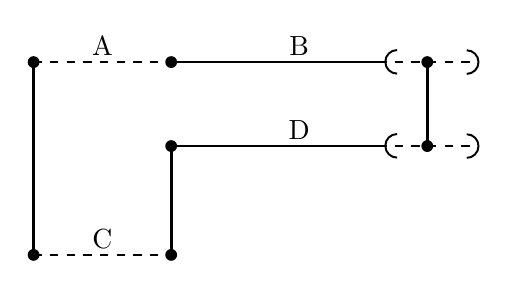
\begin{tikzpicture}
\fill (0, 21.9925) circle (0.075) ; % State.rica19 
\fill (1.74751, 21.9925) circle (0.075) ; % State.bras98 
\fill (5, 21.9925) circle (0.075) ; % State.pang86 
\fill (0, 19.5439) circle (0.075) ; % State.loge77 
\fill (1.74751, 19.5439) circle (0.075) ; % State.puma47 
\fill (1.74751, 20.926) circle (0.075) ; % State.adds96 
\fill (5, 20.926) circle (0.075) ; % State.cuny25 
\draw[line width=1pt] (0, 21.9925)  -- (0, 19.5439) ; % Sync.start 
\draw[line width=1pt] (1.74751, 21.9925)  -- (1.74751, 21.9925) ; % Sync.drip28 
\draw[line width=1pt] (5, 21.9925)  -- (5, 20.926) ; % Sync.posy23 
\draw[line width=1pt] (1.74751, 20.926)  -- (1.74751, 19.5439) ; % Sync.brew32 
\draw[dashed,line width=1pt] (0, 21.9925)  -- (1.74751, 21.9925) ; % Interval.zone49 
\draw (0.873756, 22.1925) node {A}; % Interval.zone49 
\draw[line width=1pt] (1.74751, 21.9925)  -- (4.3768, 21.9925) ; % Interval.sloe49 
\draw[dashed,line width=1pt] (4.3768, 21.9925)  -- (5.6505, 21.9925) ; % Interval.sloe49 
\draw[line width=0.7pt] (4.6168, 22.1455) arc(90:270:0.15) ; % Interval.sloe49 
\draw[line width=0.7pt] (5.5005, 21.8425) arc(-90:90:0.15) ; % Interval.sloe49 
\draw (3.37376, 22.1925) node {B}; % Interval.sloe49 
\draw[dashed,line width=1pt] (0, 19.5439)  -- (1.74751, 19.5439) ; % Interval.mayo96 
\draw (0.873756, 19.7439) node {C}; % Interval.mayo96 
\draw[line width=1pt] (1.74751, 20.926)  -- (4.3768, 20.926) ; % Interval.jura15 
\draw[dashed,line width=1pt] (4.3768, 20.926)  -- (5.6505, 20.926) ; % Interval.jura15 
\draw[line width=0.7pt] (4.6168, 21.079) arc(90:270:0.15) ; % Interval.jura15 
\draw[line width=0.7pt] (5.5005, 20.776) arc(-90:90:0.15) ; % Interval.jura15 
\draw (3.37376, 21.126) node {D}; % Interval.jura15 
\end{tikzpicture}
\caption{A given score}
\end{subfigure}~
\begin{subfigure}{0.45\textwidth}
\centering
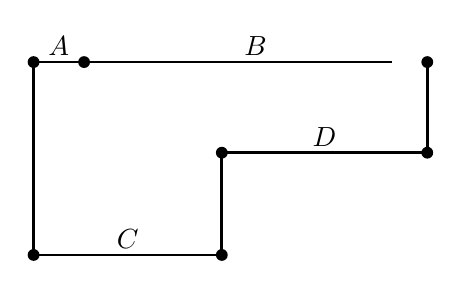
\begin{tikzpicture}
\fill (0, 21.7054) circle (0.075) ; % State.rica19 
\fill (0.641399, 21.7054) circle (0.075) ; % State.bras98 
\fill (5, 21.7054) circle (0.075) ; % State.pang86 
\fill (0, 19.256) circle (0.075) ; % State.loge77 
\fill (2.39067, 19.256) circle (0.075) ; % State.puma47 
\fill (2.39067, 20.5545) circle (0.075) ; % State.adds96 
\fill (5, 20.5545) circle (0.075) ; % State.cuny25 
\draw[line width=1pt] (0, 21.7054)  -- (0, 19.256) ; % Sync.start 
\draw[line width=1pt] (0.641399, 21.7054)  -- (0.641399, 21.7054) ; % Sync.drip28 
\draw[line width=1pt] (5, 21.7054)  -- (5, 20.5545) ; % Sync.posy23 
\draw[line width=1pt] (2.39067, 20.5545)  -- (2.39067, 19.256) ; % Sync.brew32 
\draw[line width=1pt] (0, 21.7054)  -- (0.641399, 21.7054) ; % Interval.zone49 
\draw (0.3207, 21.9054) node {$A$}; % Interval.zone49 
\draw[line width=1pt] (0.641399, 21.7054)  -- (4.55139, 21.7054) ; % Interval.sloe49 
\draw (2.8207, 21.9054) node {$B$}; % Interval.sloe49 
\draw[line width=1pt] (0, 19.256)  -- (2.39067, 19.256) ; % Interval.mayo96 
\draw (1.19534, 19.456) node {$C$}; % Interval.mayo96 
\draw[line width=1pt] (2.39067, 20.5545)  -- (5, 20.5545) ; % Interval.jura15 
\draw (3.69534, 20.7545) node {$D$}; % Interval.jura15 
\end{tikzpicture}
\caption{A trace of execution for this score: B stops executing early since its max was reached}
\end{subfigure}
\caption{A problematic case. A and C can have different durations during the execution, but the end of B and D are synchronized. In this case, the choice made is to stop executing the intervals that reached their max duration, and keep executing the others until their reach their min. The other alternative would be to keep the max constraint.}
\label{fig.maybe-incoherent}
\end{figure}

\todo{Expliquer comment on évite les deadlocks: notamment, on progresse toujours dans les autres contraintes même si on arrive au max}

\subsubsection{General execution algorithm}

* Main score and sub-scores: main score only triggers once. 
* Convenience: Sub-scores can always re-trigger and be restarted.

% \begin{algorithmic}
% \Function{ExecuteTemporalCondition}
% \EndFunction
% \Function{RunInterval}{itv, tick}
%   Add last node to ending node set
%   \If(The interval is infinite)
%     \Let{$d$}{$\min$ tick (itv.max - itv.date)}
%     Add over-tick 
%   \Else
%   \Endif
% \EndFunction
% \Function{Tick}{tick}
%   Check roots
%   Check and execute waiting temporal conditions
%   Advance running intervals
%   \Do 
%     \For(All the newly happened instantaneous conditions)
%       Advance following running intervals
%     Check and execute all finished temporal conditions
%   \While{At least a temporal condition did execute}
% \EndFunction
% \end{algorithmic}
\subsection{Loop}\label{sec.loop}
The first idea for loops would be to create a cycle in the scenario graph presented earlier.
However, acyclicity of this graph is a desirable property: this allows to keep the complexity of graph traversal operations used lower,
which matters in a real-time execution context.

Hence, we chose instead to model the loop as its own process with simpler semantics: 
a single time interval will loop. Since intervals can contain other processes, we can still encounter complex musical behaviour in it:
whole scenarios can loop.

A loop is simply defined as : 
\begin{lstlisting}
type loop = {
  itv: interval
  startTc: temporalCondition; 
  endTc: temporalCondition;
}
\end{lstlisting}

At each tick of the loop, the interval is itself executed.
If either of the temporal conditions is interactive, we follow the same process than for the scenario: 
we wait until the next tick to perform the triggering instead of doing it immediately. 
Else, further tokens are added to the interval and its child processes, starting from zero.
An example of this process is given in fig.~\ref{fig.loopautom}.

Null loop durations are prevented at creation time: else, any tick operation would cause an infinite loop since there 
would never be any progression in the loop.

\subsection{Conclusion}

\section{Data model}\label{sec.datamodel}
=> set date
=> set offset pour offset audio (p-ê pas nécessaire si on fait comme LAStream)
\todo{Canaux audio: comme Jamoma ; groupés (vs comme Max / Pd ou chaque canal a son cable)}
% \todo{Opérateurs de mixage / démixage}
% TODO pourquoi ne pas juste avoir des process "traitement du signal" flottants dans le viewport ? bof pour la gestion du temps

\section{Data graph}

\subsection{Structures}
\begin{lstlisting}
type edgeId = EdgeId of int;;
type nodeId = NodeId of int;;
type portId = PortId of int;;
type edgeType =
    Glutton
  | Strict
  | DelayedGlutton of value list
  | DelayedStrict of value list
;;
type edge = {
    edgeId: edgeId;
    source: portId;
    sink: portId;
    edgeType: edgeType;
};;
type port = {
    portId: portId;
    portAddr: string option;
    portEdges: edgeId list;
};;
type token_request = {
  token_date: duration;
  position: position;
  offset: duration;
};;
type dataNode =
    Automation of automation
  | Mapping of mapping
  | Sound of sound
  | Passthrough of passthrough;;
type grNode = {
    nodeId: nodeId;
    data: dataNode;
};;
type graph = {
    nodes: grNode list;
    edges: edge list;
};;
type grNodeState = {
  executed: bool;
  prev_date: duration;
  tokens: token_request list
};;
type graph_state = {
    node_state: (nodeId * grNodeState) list;
    port_state: (portId * value option) list
};;
\end{lstlisting}


\subsection{Operations}
Input mix on each port

\begin{lstlisting}
let init_port (p:port) g gs (e:environment) =

let init_node n g gs (e:environment) =

let write_port p (g:graph) (gs:graph_state) (e:environment) =

let teardown_node n g gs e =
\end{lstlisting}



\subsection{Tick description}

General flow: 

disable strict nodes

sort remaining nodes according to the custom order chosen (default, temporal, custom)

priority: 
* explicit cables
* local or global address

do a tick: 

\begin{lstlisting}

let rec sub_tick graph gs nodes (e:environment) =
\end{lstlisting}


\subsection{Data nodes}
Say that in the C++ code, the port kinds are statically checked : no way to mistake input from output.
\begin{lstlisting}
type curve = float -> float;;
type automation = port * curve;;
type mapping = port * port * curve;;
type sound = port * float array array;;
type passthrough = port * port;;
\end{lstlisting}
\subsubsection{Passthrough}
-> used for scenario and interval
-> mixing at the input

\begin{itemize}
\item Automation: 
start point + set of (segment * breakpoint)

tween

curve + message output port
$x\in[0;1]$ -> in the nominal duration of the parent time interval.

\item Mapping: message input port + curve + message output port
\item Javascript:  n message input port + curve + n message output port
\item Piano roll:  notes + midi output port
\item Sound file: sound data + midi output port
\item Passthrough:
\item Buffer: Used to keep audio input in memory
\item Metronome: 
\item Constant: writes a value at each tick
Why isn't the delay cable not enough ? can't go backwards. 
pb: pauser au milieu: coupure. cas dans les boucles: on réécrit par dessus (buffer vidé sur start).
\item Shader
\end{itemize}


\section{Combined model}
-> on ajoute node aux tc

-> nodeprocess fait le lien entre graphnode et time process, permet de faire l'activation et l'écoulement du temps

-> offset nécessaire pour tc pour gérer l'audio (mais pourrait être ajouté dans le modèle de base. Ou bien passer une paire de pointeurs.. ? )

\subsection{Combined tick and general flow}
Exécution complète d'un tick: 
Copy audio buffers and input data, execute the temporal tick, apply the function to the graph state, execute the graph tick, copy the output audio buffer and apply the produced state by pushing the values.


Pour être propre, il faudrait faire un "pull" général au début...

\begin{lstlisting}
let add_tick_to_node nodeId token (gs:graph_state) =
;;
\end{lstlisting}

Multiple possibilities for a tradeoff between accuracy and performance: 
\begin{itemize}
	\item Use the requested ticks. This allows to have a better the performance - latency ratio at the expense of sample-accuracy for the control data.
	\item Use the requested ticks and tick all the nodes at the smallest granularity: 
	given two nodes A, B, with tokens at $t=10$, $t=25$ for A and $t=17$ for B, tick all the nodes at 10, 17, 25.
	\item Maximal accuracy : tick with a granularity of one sample every time.
\end{itemize}



\begin{lstlisting}
let main_loop root graph duration granularity 
			  (state:score_state) ext_events ext_modifications =

\end{lstlisting}

\todo{Détailler l'approche réactive}


\subsection{Details}

Conditions et cie: The most common case for an expression is to be true.

UI: création automatique de liens implicites des enfants vers les parents si demandé (propriété de l'ui "propagate").
N'a de sens que pour l'audio de par la nature homogène de ces flux.
=> "cable créé par défaut" quand on rajoute un processus dont on marque l'entrée

=> pour toute contrainte, pour tout scénario, créer noeud qui fait le mixage
=> création d'objets récursivement, etc

- Problème des states dans scénario ?
=> states du scénario: comment interviennent-ils ? faire un scénario fantôme 


- Mettre l'accent sur la recréation de la sémantique de i-score à partir du graphe: 
=> messages: actuellement "peu" typés ; rajouter type de l'unité ? 

=> pbq du multicanal: pour l'instant non traitée, on ne gère que les cas mono / stereo pour le upmix / downmix
Choix pour multicanal: faire comme jamoma avec objets tilde
=> sliders et dispatching de canaux ?
=> cables: rubberband ? il faut mettre un rubberband dès qu'on a une entrée et une sortie qui n'ont pas la même vitesse relative. Dire que pour les automations ça interpole de manière naturelle avec le ralentissement et l'accélération (on sépare vitesse et granularité)


- Dire qu'on pourrait affiner en combinant plus précisément les "sous-ticks" temporels et de données
pour que par exemple la production d'un état dans un scénario entraîne une condition dans un autre scénario -> tout réduire à un tick

\section{Audio behaviour}

\begin{figure}[h]
\centering
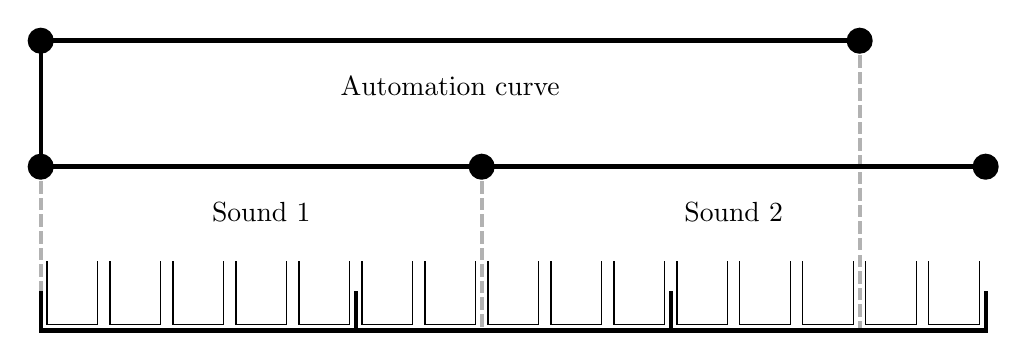
\begin{tikzpicture}[scale=0.8,line cap=rect]
  \tikzstyle{event}=[circle,thick,fill=black];
  
  % gray dashes
  \draw [dashed, line width = 1.5, opacity=0.3] (0, 9) -- (0, 6.4) ;
  \draw [dashed, line width = 1.5, opacity=0.3] (7, 9) -- (7, 6.4) ;
  \draw [dashed, line width = 1.5, opacity=0.3] (13, 11) -- (13, 6.4) ;
  \draw [line width = 1.5, opacity=1] (0, 11) -- (0, 9) ;
    
  % automation
  \coordinate (astart) at (0, 11);
  \coordinate (aend) at (13, 11);
  \draw [line width=2] (astart) -- (aend) node[midway,below,yshift=-3mm] {Automation curve};
  \node[event] at (astart) {};
  \node[event] at (aend) {};
  
  % sounds
  \coordinate (cstart) at (0, 9);
  \coordinate (cmid) at (7, 9);  
  \coordinate (cend) at (15, 9);    
  \draw [line width=2] (cstart) -- (cmid) node[midway,below,yshift=-3mm] {Sound 1};
  \draw [line width=2] (cmid) -- (cend) node[midway,below,yshift=-3mm] {Sound 2};
  \node[event] at (cstart) {};
  \node[event] at (cmid) {};
  \node[event] at (cend) {};
  
  
  % samples
  \foreach \x in {0,...,14}
    \draw [](0.1+\x, 7.5cm) -- (0.1+\x,6.5cm) -- (0.9+\x, 6.5cm) -- (0.9+\x,7.5cm);
  
  % ticks
  \foreach \x in {0,5,...,15}
    \draw [line width=1.5](\x, 6.4cm) -- (\x, 7cm) node[] {};
  \draw [line width=1.5](0, 6.4cm) -- (15, 6.4cm);
\end{tikzpicture}
\caption{A scenario. The small bins represent individual audio samples ; the bigger bins represent the tick rate of the sound card. For the sake of the example, one can assume that the automation curve is used to control the output volume of the englobing scenario, not represented here.}
\label{fig.scenarautom}
\end{figure}~
\begin{table}[h]
\centering
\begin{tabular}{c|c|c|c|c}
 & Start & Tick 1 & Tick 2 & Tick 3 \\ 
\hline 
\textbf{Automation} & $(0 \rightarrow 0, 0)$ &  &  &  \\ 
\textbf{Sound 1} & $(0 \rightarrow 0, 0)$ & $(0 \rightarrow 5, 0)$ & $(5 \rightarrow 7, 0)$ &  \\ 
\textbf{Sound 2} &  &  & $(0 \rightarrow 3, 2)$ & $(3 \rightarrow 8, 0)$ \\ 
\textbf{Scenario} & $(0 \rightarrow 0, 0)$ & $(0 \rightarrow 5, 0)$ & $(5 \rightarrow 10, 0)$ & $(10 \rightarrow 15, 0)$ \\ 
\end{tabular} 
\caption{Value of token requests for the scenario ~\ref{fig.scenarautom}. The tokens are written as (previous date $\rightarrow$ current date, offset).}
\end{table}



\tikzstyle{flexinterv}=[dash pattern=on 8pt off 4pt];
\begin{figure}[h]
\centering
\begin{tikzpicture}[scale=0.8,line cap=rect]
  \tikzstyle{event}=[circle,thick,fill=black];
  
  % gray dashes
  \draw [dashed, line width = 1.5, opacity=0.3] (0, 9) -- (0, 6.4) ;
  \draw [dashed, line width = 1.5, opacity=0.3] (7, 9) -- (7, 6.4) ;
    
  % sounds
  \coordinate (cstart) at (0, 9);
  \coordinate (cflex) at(3, 9);
  \coordinate (cmid) at (7, 9);  
  \coordinate (cend) at (15, 9);
  \draw [line width=0,draw=none] (cstart) -- (cmid) node[midway,below,yshift=-3mm] {Sound 1};
  \draw [line width=2] (cstart) -- (cflex);
  \draw [line width=2,flexinterv] (cflex) -- (cmid);
  \draw [line width=2] (cmid) -- (cend) node[midway,below,yshift=-3mm] {Sound 2};
  
  \draw [line width=2] ([shift={(3.3,9)}] 90:0.3) arc[radius=0.3, start angle=90, end angle=270] ;
  \node[event] at (cstart) {};
  \node[event] at (cmid) {};
  \node[event] at (cend) {};
  
  
  % samples
  \foreach \x in {0,...,14}
    \draw [](0.1+\x, 7.5cm) -- (0.1+\x,6.5cm) -- (0.9+\x, 6.5cm) -- (0.9+\x,7.5cm);
  
  % ticks
  \foreach \x in {0,5,...,15}
    \draw [line width=1.5](\x, 6.4cm) -- (\x, 7cm) node[] {};
  \draw [line width=1.5](0, 6.4cm) -- (15, 6.4cm);
  

  % event  
  \draw [dashed, line width = 3, color=orange] (5.7, 9.5) -- (5.7, 8.5)
        node[above,yshift=8mm] {An external event happens} ;
\end{tikzpicture}
\caption{A scenario with an interaction.}
\label{fig.scenarinteract}
\end{figure}~
\begin{table}[h]
\centering
\begin{tabular}{c|c|c|c|c}
 & Start & Tick 1 & Tick 2 & Tick 3 \\ 
\hline 
\textbf{Sound 1} & $(0 \rightarrow 0, 0)$ & $(0 \rightarrow 5, 0)$ & $(5 \rightarrow 10, 0)$ & \\ 
\textbf{Sound 2} &  &  &  & $(0 \rightarrow 5, 0)$ \\ 
\textbf{Scenario} & $(0 \rightarrow 0, 0)$ & $(0 \rightarrow 5, 0)$ & $(5 \rightarrow 10, 0)$ & $(10 \rightarrow 15, 0)$ \\ 
\end{tabular} 
\caption{Value of token requests for the scenario~\ref{fig.scenarinteract}.}
\end{table}


\begin{figure}[h]
\centering
\begin{tikzpicture}[scale=0.8,line cap=rect]
  \tikzstyle{event}=[circle,thick,fill=black];
  
  % gray dashes
  \draw [dashed, line width = 1.5, opacity=0.3] (0, 9) -- (0, 6.4) ;
  \draw [dashed, line width = 1.5, opacity=0.3] (7, 9) -- (7, 6.4) ;
  \draw [dashed, line width = 1.5, opacity=0.3] (14, 9) -- (14, 6.4) ;
  \draw [line width = 1.5, opacity=1] (0, 11) -- (0, 9) ;
    
  % loop
  \coordinate (cstart) at (0, 11);
  \coordinate (cend) at (15, 11);    
  \draw [line width=2,flexinterv] (cstart) -- (cend) node[midway,below,yshift=-3mm] {Loop};
  \node[event] at (cstart) {};
  
  % pattern  
  \coordinate (lstart) at (0, 9);
  \coordinate (lend) at (7, 9);  
  \draw [line width=2] (lstart) -- (lend) node[midway,below,yshift=-3mm] {Loop pattern (sound)};
      
  % repetition
  \coordinate (rstart) at (7, 9);
  \coordinate (rend) at (14, 9); 
  \coordinate (rend2) at (15, 9);  
  \draw [line width=2, color=gray] (rend) -- (rend2);    
  
  \draw [line width=2, color=gray] (rstart) -- (rend) node[midway,below,yshift=-3mm] {Repetition};    
  \node[event] at (lstart) {};   
  \node[event] at (lend) {}; 
  \node[event, color=gray] at (rend) {};
  
  % samples
  \foreach \x in {0,...,14}
    \draw [](0.1+\x, 7.5cm) -- (0.1+\x,6.5cm) -- (0.9+\x, 6.5cm) -- (0.9+\x,7.5cm);
    
  % ticks
  \foreach \x in {0,5,...,15}
    \draw [line width=1.5](\x, 6.4cm) -- (\x, 7cm) node[] {};
  \draw [line width=1.5](0, 6.4cm) -- (15, 6.4cm);
\end{tikzpicture}
\caption{A loop containing a sound.}
\label{fig.loopautom}
\end{figure}~
\begin{table}[h]
\centering
\begin{tabular}{c|c|c|c|c}
 & Start & Tick 1 & Tick 2 & Tick 3 \\ 
\hline 
\textbf{Pattern} & $(0 \rightarrow 0, 0)$ & $(0\rightarrow 5, 0)$ & $(5\rightarrow 7, 0), (0 \rightarrow 3, 2)$ & $(3 \rightarrow 7, 0), (0 \rightarrow 1, 4)$ \\ 
\textbf{Loop} & $(0 \rightarrow 0, 0)$ & $(0 \rightarrow 5, 0)$ & $(5 \rightarrow 10, 0)$ & $(10 \rightarrow 15, 0)$ \\ 
\end{tabular} 
\caption{Value of token requests for the scenario~\ref{fig.loopautom}}
\end{table}

Expliquer tick avec données, offset, etc.

Cas complexe: 

dernier tick d'une boucle qui a un enfant fichier son + automation



\section{Mapping from visual language}
All the objects in the visual language correspond to the objects presented earlier, at the exception of the states.

States : intervals with a duration equal to zero.
IC / TC / interval / processes : no change
edges : between processes
\section{Applications and examples}

\subsection{Reconstructing existing paradigms}\label{sec.existingparadigms}
In this part we give example of reconstruction of standard audio software behaviours with the given model.
\subsubsection{Audio sequencer}
Notable software in this category includes Steinberg Cubase, Avid Pro Tools, \dots

The common metaphor for audio sequencers is the track, inspired from mixing desks and tape recorders. 
We will take the example of audio and midi tracks. 
Such an audio sequencer can be modeled by : 

\begin{itemize}
    \item A root: an infinite interval.
    \item This interval contains two processes: a scenario and an effect bus. 
    The sound output of the scenario goes to the input of the effect bus.
    \item The scenario contains the actual tracks.
    \item These tracks are also modeled by infinite constraints.
\end{itemize}

We divide the tracks in two categories.
Audio tracks are built with : 
\begin{itemize}
  \item A scenario with a single sequence of intervals, some of which may bear sound file processes and others being empty.
  \item An effect bus process. The output of the scenario goes to the input of the effect bus. Generally, this effect bus would end by channel operations such as panning and volume adjustment, in a similar fashion to mixing desks.
\end{itemize} 

Midi tracks are built with : 
\begin{itemize}
    \item A scenario with a single sequence of intervals, some of which may bear MIDI notes processes and others being empty.
    \item An instrument process, which takes MIDI data and outputs sound.
    \item Like before, an effect bus applied to the instrument's output.
\end{itemize}

This can easily be extended with further features: sends, automations, etc.
\subsubsection{Looping audio sequencer}
More recently, a different kind of sequencer has emerged: the looping, non-linear sequencer. 
The prime example of this is Ableton Live. We give the example for a simplified model of live-looping without quantization.

These sequencers are also organized in tracks ; however, within a track, the musician can choose a single loop 
that is currently playing, and regularly switch the current loop.

Hence, the general organization stays the same than for the audio sequencer: most importantly, the way effect buses are applied does not change.

\begin{itemize}
    \item Each clip of a track is given an index. 
    \item Each track also has a parameter which is the next clip to play, \lstinline|next_clip|. These parameters can be introduced as variables in the device tree.
    \item We replace the scenarios containing the actual sound files or midi notes by loop processes. 
    \item The loops processes are defined with and ending temporal condition. 
    \item Inside the loop pattern, there is a single scenario process. This scenario process has a set of parallel intervals, each with one sound file. Every interval begins with an instantaneous condition that compares the \lstinline|next_clip| parameter to the current clip's index. Hence, at most one clip is playing at the same time in each track. If the \lstinline|next_clip| does not change the track keeps looping on the sound file.
\end{itemize}

Extension: par ex. dans une boucle on peut mettre un autre scénario.
Pb : tic qui manque. On peut y remédier en exécutant le trigger "en avance".
\subsubsection{Patcher}


\subsection{Musical examples}
\subsubsection{Audio compositing}
-> on utilise un scénario qui lit des parties d'une entrée son dans différents bus d'effets. L'effet peut se déclencher en retard.

Org: 

Intervalle racine

Process 1:  Audio input
Process 2 : Scenario
  -> Trois itv ; entrée reliée strict à sortie de audio input ; sortie dans parent
  
Process 3 : FX
Process 4 : scenario
Audio Input -> itv {1,2,3} -> scenario -> fx -> scenario

\subsection{Notes on implementation}


=> "third gen" audio sequencer.
first gen: cubase, etc
second gen: non-linear: ableton, bitwig
third gen: entirely interactive: i-score, iannix. what else ? 

reproducibilité: code source dispo

type-safety de l'écriture des nœuds

réimplémentation de la séparation controle / input par dessus.

algorithme qui séquence les contrôles

messages: sample accurate ; par tick, on ordonnance pour un nœud donné


\section{Evaluation and Discussion}
Enforcing graph constraints: mostly done through UI. For instance: ic are created on tc, etc. No "going back" which would break DAG-ness.

Faire parenthèse sur domain driven design sur logiciels de musique qui fournit de meilleurs résultats que application directe de modèles existants (petri, etc).
Peut-être donner un méta-modèle qui correspond à nos structures ?

Dire pourquoi un tic est introduit lors d'une interaction (notamment, permet de ne pas avoir de "boucle infinie" si on a une boucle de durée 0 avec deux triggers vrais) ; est aussi plus cohérent pour les utilisateurs pour qui une interaction doit être manifeste.

Avantage: manipulation uniforme des processus, que ce soit des automations, des groupes, des fichiers sons, etc.
\section{Conclusion}

missing: quantification

missing: sound speed


\bibliography{biblio}

\end{document}